\documentclass[uplatex]{jsarticle}

\usepackage[dvipdfmx]{graphicx}
\usepackage[dvipdfmx]{color}
\usepackage{caption}
\usepackage{float}

\setlength{\textheight}{244truemm}
\setlength{\headheight}{0pt}
\setlength{\headsep}{25truemm}
\setlength{\footskip}{15truemm}
\addtolength{\topmargin}{-1truein}

\begin{document}
	\section{目的}
		電気回路は電圧を加えた瞬間や,切った瞬間は定常とは異なった動作をする.この時に起こる現象を過度現象といい,有害な時もあるが,
		電子回路などでは今原理を利用することも多い.\par
		ここでは,直流の場合の$R$と$C$の直列回路の充電$\cdot$放電特性を測定することを通して, RC回路に生ずる過度現象とその時定数を知る.
	\section{理論}
		コンデンサに電流が流れ込むと電荷が蓄えられる.コンデンサの端子間の電圧を測定してみれば,その様子を間接的に見ることができる.
		電荷が何も蓄えられていない時は, $0 [\mathrm V]$であるし,少しでも蓄えられていれば,幾らかの電圧が測定されるはずである.\\[1ex]
		\ \ \ 図1の充電を考える. $S$をONにし,電圧を加えると$C$に電流が流れて充電が始まる.時間が十分経過して,コンデンサの電圧$V_{C}$が電源の電圧$E$と等しくなると充電
		が終わり,電流が流れなくなる.
		\begin{figure}[H]
			\begin{minipage}{0.5\hsize}
				\begin{center}
					\includegraphics[width = 7cm]{1-a.eps}
				\end{center}
				\captionsetup{labelformat=empty,labelsep=none}
				\caption{a. RC回路}
			\end{minipage}
			\begin{minipage}{0.5\hsize}
				\begin{center}
					\includegraphics[width = 5cm]{1-b.eps}
				\end{center}
				\captionsetup{labelformat=empty,labelsep=none}
				\caption{b. 電流・電圧}
			\end{minipage}
			\captionsetup{labelformat=empty,labelsep=none}
			\caption{図1: コンデンサの充電}
		\end{figure}
		また,図2は電圧として$E(=V_{C})$充電されたコンデンサの放電の様子を表している. $V_{C}$が$0 [\mathrm V]$になると,放電が終わり電流が流れなくなる.
		\begin{figure}[H]
			\begin{minipage}{0.5\hsize}
				\begin{center}
					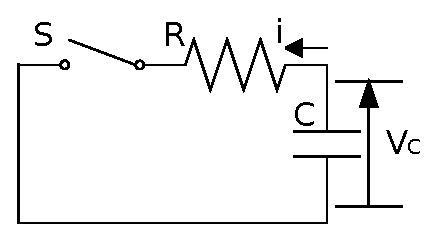
\includegraphics[width = 7cm]{2-a.eps}
				\end{center}
				\captionsetup{labelformat=empty,labelsep=none}
				\caption{a. RC回路}
			\end{minipage}
			\begin{minipage}{0.5\hsize}
				\begin{center}
					\includegraphics[width = 5cm]{2-b.eps}
				\end{center}
				\captionsetup{labelformat=empty,labelsep=none}
				\caption{b. 電流・電圧}
			\end{minipage}
			\captionsetup{labelformat=empty,labelsep=none}
			\caption{図2: コンデンサの放電}
		\end{figure}
		「コンデンサは直流を通さない」と表現することがある.これは電圧を加えてから十分時間が経過後(定常状態),充電や放電が終わった後のことを言っている.
		ここの例のように,電圧を加えた瞬間は定常状態の時とは異なる動作となる.\par
		当然,充電放電が速ければ,早くに定常状態となり得る.
		\begin{figure}[H]
			\begin{minipage}{0.5\hsize}
				\begin{center}
					\includegraphics[width = 6cm]{3-a.eps}
				\end{center}
				\captionsetup{labelformat=empty,labelsep=none}
				\caption{a. 充電}
			\end{minipage}
			\begin{minipage}{0.5\hsize}
				\begin{center}
					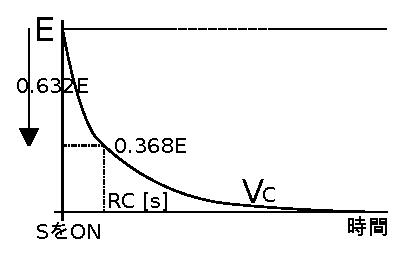
\includegraphics[width = 6cm]{3-b.eps}
				\end{center}
				\captionsetup{labelformat=empty,labelsep=none}
				\caption{b. 放電}
			\end{minipage}
			\captionsetup{labelformat=empty,labelsep=none}
			\caption{図3: コンデンサの電圧変化}
		\end{figure}
		充放電の速さは$R \times C \ [\mathrm s]$で決まる. $R \times C$を時定数といい$\tau$(タウ)で表す.\par
		RC回路の充放電において,時定数$\tau$経過後のコンデンサの電圧は,最終値の$63.2 \%$の値に達する. $R$や$C$がそれぞれ異なっている回路でも$\tau$が等しければ,
		同様な動作をする.
	\section{実験}
		図4はRC回路の充放電特性を測定する回路である. $R$と$C$はブレッドボード上で接続する.\par
		スイッチ$S$は中心位置ではどこにも接続されない.また,スイッチ$S$は充電特性を測定する時はグランド側,放電特性を測定する時には直流電源側に接続されるように設定する.
		\begin{figure}[h]
			\begin{center}
				\includegraphics{4.eps}
			\end{center}
			\captionsetup{labelformat=empty,labelsep=none}
			\caption{図4: RC回路の充放電特性}
		\end{figure}
		\subsection{測定}
			RC回路充電放電特性の測定結果として図5のような結果が欲しい.充電特性の測定,放電特性の測定の順で行う.
			\paragraph{充電特性}
			\begin{enumerate}
				\item{$R = 47 \ [\mathrm k \Omega], C = 1000 \ [\mathrm \mu F]$で回路を組み接続する.}
				\item{直流電源の電圧を$E = 10 [\mathrm V]$に設定する.}
				\item{スイッチ$S$をグランド側に接続されるように設定し,コンデンサの電圧が$0 [\mathrm V]$}
				\item{スイッチ$S$を直列電源側に接続されるように接続する.同時にストップウォッチをスタートさせる.}
				\item{コンデンサの電圧が,$1,2,\cdot\cdot\cdot,9,10 \ [\mathrm V]$になった時の時間を測定し,表1の様にまとめる.}
				\item{$R$,$C$の組み合わせを次の様に変えて,測定を繰り返す.\\
					$R = 22 \ [\mathrm k \Omega], C = 2200 \ [\mathrm \mu F] \quad R = 68 \ [\mathrm k \Omega], C = 1000 \ [\mathrm \mu F] \quad R = 33 \ [\mathrm k \Omega], C = 2200 \ [\mathrm \mu F]$}
			\end{enumerate}
			\paragraph{放電特性}
			\begin{enumerate}
				\setcounter{enumi}{6}
				\item{$R = 47 \ [\mathrm k \Omega], C = 1000 \ [\mathrm \mu F]$で回路を組み接続する.}
				\item{直流電源の電圧を$E = 10 [\mathrm V]$に設定する.}
				\item{スイッチ$S$を直列電源側に接続されるように設定し,コンデンサの電圧が$0 [\mathrm V]$}
				\item{スイッチ$S$をグランド側に接続されるように接続する.同時にストップウォッチをスタートさせる.}
				\item{コンデンサの電圧が,$10,9,\cdot\cdot\cdot,1,0 \ [\mathrm V]$になった時の時間を測定し,表2の様にまとめる.}
				\item{$R$,$C$の組み合わせを次の様に変えて,測定を繰り返す.\\
					$R = 22 \ [\mathrm k \Omega], C = 2200 \ [\mathrm \mu F] \quad R = 68 \ [\mathrm k \Omega], C = 1000 \ [\mathrm \mu F] \quad R = 33 \ [\mathrm k \Omega], C = 2200 \ [\mathrm \mu F]$}
			\end{enumerate}
			直流電源: Ec-06 \quad マルチメーター: Ec-13
		\subsection{測定結果}
			\begin{figure}[h]
				\begin{minipage}{0.5\hsize}
					\begin{center}
						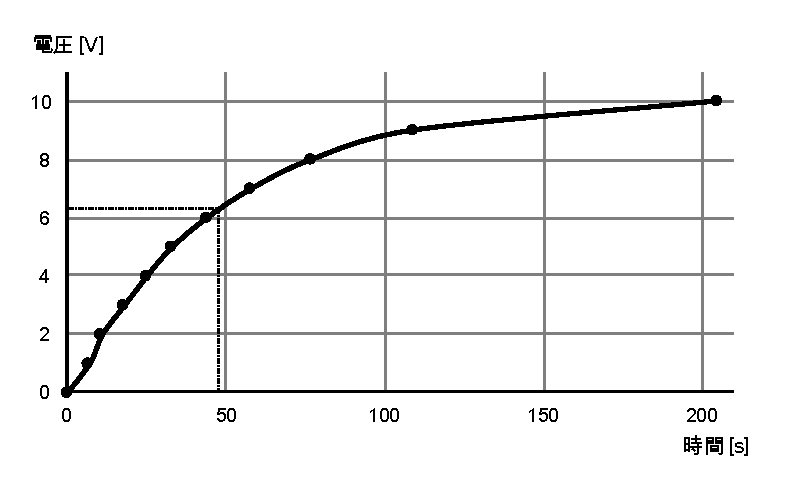
\includegraphics[width = 8cm]{5-a.eps}
					\end{center}
					\captionsetup{labelformat=empty,labelsep=none}
					\caption{a. 充電特性}
				\end{minipage}
				\begin{minipage}{0.5\hsize}
					\begin{center}
						\includegraphics[width = 8cm]{5-b.eps}
					\end{center}
					\captionsetup{labelformat=empty,labelsep=none}
					\caption{b. 放電特性}
				\end{minipage}
				\captionsetup{labelformat=empty,labelsep=none}
				\caption{図5: RC回路の特性}
			\end{figure}
			\begin{figure}[h]
				\begin{minipage}{0.5\hsize}
					\begin{center}
						\includegraphics[width = 8cm]{6-a.pdf}
					\end{center}
					\captionsetup{labelformat=empty,labelsep=none}
					\caption{a. 充電特性 $\tau$測定値 = 49 [s]}
				\end{minipage}
				\begin{minipage}{0.5\hsize}
					\begin{center}
						\includegraphics[width = 8cm]{6-b.pdf}
					\end{center}
					\captionsetup{labelformat=empty,labelsep=none}
					\caption{b. 放電特性 $\tau$測定値 = 50 [s]}
				\end{minipage}
				\captionsetup{labelformat=empty,labelsep=none}
				\caption{図6: $R = 47 \ [\mathrm k \Omega], C = 1000 \ [\mathrm \mu F], \tau \ 理論値 = 47 \ [\mathrm s]$}
			\end{figure}
			\begin{figure}[h]
				\begin{minipage}{0.5\hsize}
					\begin{center}
						\includegraphics[width = 8cm]{7-a.pdf}
					\end{center}
					\captionsetup{labelformat=empty,labelsep=none}
					\caption{a. 充電特性 $\tau$測定値 = 58 [s]}
				\end{minipage}
				\begin{minipage}{0.5\hsize}
					\begin{center}
						\includegraphics[width = 8cm]{7-b.pdf}
					\end{center}
					\captionsetup{labelformat=empty,labelsep=none}
					\caption{b. 放電特性 $\tau$測定値 = 51 [s]}
				\end{minipage}
				\captionsetup{labelformat=empty,labelsep=none}
				\caption{図7: $R = 22 \ [\mathrm k \Omega], C = 2200 \ [\mathrm \mu F], \tau \ 理論値 = 48.4 \ [\mathrm s]$}
			\end{figure}
			\begin{figure}[h]
				\begin{minipage}{0.5\hsize}
					\begin{center}
						\includegraphics[width = 8cm]{8-a.pdf}
					\end{center}
					\captionsetup{labelformat=empty,labelsep=none}
					\caption{a. 充電特性 $\tau$測定値 = 74 [s]}
				\end{minipage}
				\begin{minipage}{0.5\hsize}
					\begin{center}
						\includegraphics[width = 8cm]{8-b.pdf}
					\end{center}
					\captionsetup{labelformat=empty,labelsep=none}
					\caption{b. 放電特性 $\tau$測定値 = 68 [s]}
				\end{minipage}
				\captionsetup{labelformat=empty,labelsep=none}
				\caption{図8: $R = 68 \ [\mathrm k \Omega], C = 1000 \ [\mathrm \mu F], \tau \ 理論値 = 68 \ [\mathrm s]$}
			\end{figure}
			\begin{figure}[!h]
				\begin{minipage}{0.5\hsize}
					\begin{center}
						\includegraphics[width = 8cm]{9-a.pdf}
					\end{center}
					\captionsetup{labelformat=empty,labelsep=none}
					\caption{a. 充電特性 $\tau$測定値 = 80 [s]}
				\end{minipage}
				\begin{minipage}{0.5\hsize}
					\begin{center}
						\includegraphics[width = 8cm]{9-b.pdf}
					\end{center}
					\captionsetup{labelformat=empty,labelsep=none}
					\caption{b. 放電特性 $\tau$測定値 = 76 [s]}
				\end{minipage}
				\captionsetup{labelformat=empty,labelsep=none}
				\caption{図9: $R = 33 \ [\mathrm k \Omega], C = 2200 \ [\mathrm \mu F], \tau \ 理論値 = 72.6 \ [\mathrm s]$}
			\end{figure}
			\begin{table}[h]
				\centering
				\small
				\caption{RC回路の充電特性}
				\begin{tabular}{c|ccc|ccc|ccc|ccc} \hline \hline
					 & \multicolumn{3}{l|}{$R = 47 \ [\mathrm k \Omega]$} & \multicolumn{3}{l|}{$R = 22 \ [\mathrm k \Omega]$} & \multicolumn{3}{l|}{$R = 68 \ [\mathrm k \Omega]$} & \multicolumn{3}{l}{$R = 33 \ [\mathrm k \Omega]$} \\
					電圧 & \multicolumn{3}{l|}{$C = 1000 \ [\mathrm \mu F]$} & \multicolumn{3}{l|}{$C = 2200 \ [\mathrm \mu F]$} & \multicolumn{3}{l|}{$C = 1000 \ [\mathrm \mu F]$} & \multicolumn{3}{l}{$C = 2200 \ [\mathrm \mu F]$} \\
					$E \ [\mathrm V]$ & \multicolumn{3}{l|}{このときの時間 \ [s]} & \multicolumn{3}{l|}{このときの時間 \ [s]} & \multicolumn{3}{l|}{このときの時間 \ [s]} & \multicolumn{3}{l}{このときの時間 \ [s]} \\ \cline{2-13}
					   & 1回目 & 2回目 & 平均  & 1回目 & 2回目 & 平均  & 1回目 & 2回目 & 平均  & 1回目 & 2回目 & 平均 \\ \hline
					0  & 0.0   & 0.0   & 0.0   & 0.0   & 0.0   & 0.0   & 0.0   & 0.0   & 0.0   & 0.0   & 0.0   & 0.0 \\ \hline
					1  & 5.2   & 5.6   & 5.4   & 4.8   & 4.7   & 4.8   & 7.4   & 7.5   & 7.5   & 8.1   & 8.3   & 8.2 \\ \hline
					2  & 11.0  & 11.5  & 11.3  & 11.1  & 11.1  & 11.1  & 16.1  & 16.2  & 16.2  & 17.8  & 17.9  & 17.9 \\ \hline
					3  & 17.9  & 17.9  & 17.9  & 18.5  & 18.3  & 18.4  & 26.1  & 26.2  & 26.2  & 28.8  & 28.9  & 28.9 \\ \hline
					4  & 25.7  & 26.0  & 25.9  & 27.6  & 26.8  & 27.2  & 37.5  & 37.6  & 37.6  & 41.5  & 41.9  & 41.7 \\ \hline
					5  & 35.2  & 35.4  & 35.3  & 38.4  & 37.1  & 37.8  & 51.4  & 51.6  & 51.5  & 57.2  & 57.5  & 57.4 \\ \hline
					6  & 46.9  & 46.8  & 46.9  & 53.1  & 50.1  & 51.6  & 68.5  & 68.5  & 68.5  & 77.0  & 77.1  & 77.1 \\ \hline
					7  & 62.9  & 62.4  & 62.7  & 74.0  & 67.8  & 70.9  & 90.9  & 91.1  & 91.0  & 103.9 & 104.1 & 104.0 \\ \hline
					8  & 85.7  & 84.6  & 85.2  & 106.2 & 94.3  & 100.3 & 123.7 & 123.5 & 123.6 & 144.4 & 144.4 & 144.4 \\ \hline
					9  & 127.4 & 124.0 & 125.7 & 169.2 & 147.1 & 158.2 & 182.0 & 181.6 & 181.8 & 224.0 & 223.2 & 223.6 \\ \hline
					10 & 201.1 & 200.0 & 200.6 & 210.4 & 210.3 & 210.4 & 247.8 & 250.3 & 249.1 & 332.5 & 331.6 & 332.1 \\ \hline
				\end{tabular}
			\end{table}
			\begin{table}[h]
				\centering
				\small
				\caption{RC回路の放電特性}
				\begin{tabular}{c|ccc|ccc|ccc|ccc} \hline \hline
					 & \multicolumn{3}{l|}{$R = 47 \ [\mathrm k \Omega]$} & \multicolumn{3}{l|}{$R = 22 \ [\mathrm k \Omega]$} & \multicolumn{3}{l|}{$R = 68 \ [\mathrm k \Omega]$} & \multicolumn{3}{l}{$R = 33 \ [\mathrm k \Omega]$} \\
					電圧 & \multicolumn{3}{l|}{$C = 1000 \ [\mathrm \mu F]$} & \multicolumn{3}{l|}{$C = 2200 \ [\mathrm \mu F]$} & \multicolumn{3}{l|}{$C = 1000 \ [\mathrm \mu F]$} & \multicolumn{3}{l}{$C = 2200 \ [\mathrm \mu F]$} \\
					$E \ [\mathrm V]$ & \multicolumn{3}{l|}{このときの時間 \ [s]} & \multicolumn{3}{l|}{このときの時間 \ [s]} & \multicolumn{3}{l|}{このときの時間 \ [s]} & \multicolumn{3}{l}{このときの時間 \ [s]} \\ \cline{2-13}
					   & 1回目 & 2回目 & 平均  & 1回目 & 2回目 & 平均  & 1回目 & 2回目 & 平均  & 1回目 & 2回目 & 平均 \\ \hline
					10 & 0.0   & 0.0   & 0.0   & 0.0   & 0.0   & 0.0   & 0.0   & 0.0   & 0.0   & 0.0   & 0.0   & 0.0 \\ \hline
					9  & 3.1   & 5.5   & 4.3   & 4.8   & 4.9   & 4.9   & 6.9   & 7.1   & 7.0   & 6.3   & 7.1   & 6.7 \\ \hline
					8  & 9.1   & 11.5  & 10.3  & 11.5  & 11.6  & 11.6  & 15.5  & 15.8  & 15.7  & 16.4  & 16.6  & 16.5 \\ \hline
					7  & 16.0  & 18.4  & 17.2  & 19.2  & 19.5  & 19.4  & 25.4  & 25.7  & 25.6  & 27.9  & 28.7  & 28.3 \\ \hline
					6  & 24.0  & 25.6  & 24.8  & 27.8  & 28.2  & 28.0  & 37.0  & 37.3  & 37.2  & 41.0  & 41.8  & 41.4 \\ \hline
					5  & 33.4  & 35.7  & 34.6  & 38.5  & 38.8  & 38.7  & 50.7  & 51.0  & 50.9  & 56.8  & 57.3  & 57.1 \\ \hline
					4  & 45.4  & 47.3  & 46.4  & 51.3  & 51.6  & 51.5  & 67.3  & 67.6  & 67.5  & 76.2  & 76.9  & 76.6 \\ \hline
					3  & 60.4  & 61.7  & 61.1  & 70.7  & 68.6  & 69.7  & 88.8  & 89.0  & 88.9  & 101.5 & 102.3 & 101.9 \\ \hline
					2  & 81.4  & 82.9  & 82.2  & 100.1 & 94.3  & 97.2  & 119.1 & 119.5 & 119.3 & 139.7 & 140.0 & 139.9 \\ \hline
					1  & 116.6 & 118.2 & 117.4 & 147.4 & 145.2 & 146.3 & 170.3 & 170.5 & 170.4 & 216.0 & 215.3 & 215.7 \\ \hline
					0  & 230.0 & 219.0 & 224.5 & 210.3 & 210.4 & 210.4 & 250.3 & 250.4 & 250.4 & 330.3 & 330.3 & 330.3 \\ \hline
				\end{tabular}
			\end{table}
	\clearpage
	\section{課題$\cdot$考察}
		\begin{enumerate}
			\item{時定数は理論値一致したか.一致しないとすればどの様な原因が考えられるか.その対策はどうすれば良いか.} \\
				概ね一致した.誤差があるものでは、誤差は概ね5-10 \% ほどだった.これは,使用した抵抗が誤差率±5 \% のものを使用していたことが関係していると思われる.
			\item{時定数の大小によって特性曲線はどう変わるか.} \\
				時定数$\tau$が大きいほど,特性曲線は時間軸方向に大きくなる.
		\end{enumerate}
\end{document}
